\newpage
МРНТИ 65.63.35
\hfill {\bfseries \href{https://doi.org/10.58805/kazutb.v.3.24-570}{https://doi.org/10.58805/kazutb.v.3.24-570}}

\sectionwithauthors{А.Б. Рахматуллина, Ф.Т.Диханбаева, Д.А. Тлевлесова М.К. Изтилеуов, Б.К.
Калемшарив}{РАЗРАБОТКА И ОПТИМИЗАЦИЯ ТЕХНОЛОГИИ СУБЛИМАЦИОННОЙ СУШКИ КОБЫЛЬЕГО МОЛОКА: АНАЛИЗ СОСТАВА, МЕТОДОВ И ВЫХОДОВ ПРОДУКЦИИ}
\begin{center}
{\bfseries \textsuperscript{1}А.Б. Рахматуллина, \textsuperscript{1,
2}Ф.Т.Диханбаева, \textsuperscript{1}Д.А. Тлевлесова\envelope, }

{\bfseries \textsuperscript{2}М.К. Изтилеуов, \textsuperscript{3}Б.К.Калемшарив}

\textsuperscript{1}Институт механики и машиноведения имени академика
У.А. Джолдасбекова, Алматы, Казахстан,

\textsuperscript{2}Алматинский технологический университет, Алматы,
Казахстан,

\textsuperscript{3}Казахский агротехнический исследовательский
университет им. С. Сейфуллина, Астана, Казахстан
\end{center}

\envelope Корреспондент-автор: tlevlessova@gmail.com\vspace{0.5cm}

В статье представлено исследование по разработке и оптимизации
технологии производства сухих молочных продуктов из кобыльего молока с
использованием метода сублимационной сушки. Основ-ной целью исследования
являлось определение оптимальных условий сублимационной сушки для
максимального сохранения питательных и биологически активных компонентов
молока. В ходе экс-периментов был проведен детальный анализ
физико-химических свойств кобыльего молока, включая содержание белка,
жира, лактозы и минеральных солей. Исследовались различные температурные
режимы сублимационной сушки, чтобы определить их влияние на выход и
качество сухого молока.

Результаты показали, что оптимальная температура сушки составляет около
35°C, при которой достигается максимальный выход сухого молока с
минимальными потерями питательных веществ. Выход сухого молока составил
67.14 грамм на 600 грамм жидкого молока. Полученные данные были
сопоставлены с существующими литературными данными, что подтвердило
эффективность выбранного метода.

В статье также обсуждаются технологические параметры сублимационной
сушки и их влияние на качество конечного продукта. На основе полученных
результатов разработаны рекомендации по оптимизации процесса сушки
кобыльего молока. Дальнейшие исследования будут направлены на улучшение
технологических процессов и увеличение выхода готовой продукции.

{\bfseries Ключевые слова:} кобылье молоко, сублимационная сушка,
оптимизация технологии, питатель-ные вещества, физико-химический анализ.

\sectionheading{БИЕ СҮТІН МҰЗДАТЫП КЕПТІРУ ТЕХНОЛОГИЯСЫН ӘЗІРЛЕУ ЖӘНЕ
ОҢТАМАЛАНДЫРУ: ҚҰРАМЫН, ӘДІСТЕРІН ЖӘНЕ ӨНІМ ШЫҒЫМЫН ТАЛДАУ}
\begin{center}

{\bfseries \textsuperscript{1}А.Б. Рахматуллина,
\textsuperscript{1,2}Ф.Т.Диханбаева, \textsuperscript{1}Д.А.
Тлевлесова\envelope,}

{\bfseries \textsuperscript{2}М.Қ. Ізтілеуов, \textsuperscript{3}Б.Қ.
Қалемшарив}

\textsuperscript{1}Академик Ө.Ә. Жолдасбеков атындағы Механика және
инженерия институты, Алматы, Қазақстан,

\textsuperscript{2}Алматы технологиялық университеті, Алматы, Қазақстан,

\textsuperscript{3}С.Сейфуллина атындағы Қазақ агротехникалық зерттеу
университеті. Астана, Қазақстан,

e-mail: tlevlessova@gmail.com
\end{center}

Мақалада мұздатып кептіру әдісімен бие сүтінен құрғақ сүт өнімдерін
өндіру технологиясын жасау және оңтайландыру бойынша зерттеу берілген.
Зерттеудің негізгі мақсаты сүттің тағамдық және биологиялық белсенді
компоненттерін барынша сақтау үшін мұздату әдісімен кептірудің оңтайлы
шарттарын анықтау болды. Тәжірибе барысында бие сүтінің құрамындағы
ақуыз, май, лактоза және минералды тұздарды қамтитын физика-химиялық
қасиеттеріне егжей-тегжейлі талдау жасалды. Құр-ғақ сүттің шығымы мен
сапасына әсерін анықтау үшін мұздатып кептірудің әртүрлі температуралық
жағдайлары зерттелді.

Нәтижелер кептірудің оңтайлы температурасы 35°C шамасында екенін
көрсетті, бұл қоректік зат-тардың аз шығынымен сүт ұнтағының максималды
шығымына қол жеткізеді. Құрақ сүттің шығымы 600 грамм сұйық сүттен 67,14
грамм болды. Алынған мәліметтер таңдалған әдістің тиімділігін растай-тын
бар әдебиет деректерімен салыстырылды.

Сондай-ақ мақалада мұздатып кептірудің технологиялық параметрлері және
олардың соңғы өнім сапасына әсері қарастырылған. Алынған нәтижелер
бойынша бие сүтін кептіру процесін оңтайланды-ру бойынша ұсыныстар
әзірленді. Әрі қарайғы зерттеулер технологиялық процестерді жетілдіруге
және дайын өнімнің шығымдылығын арттыруға бағытталатын болады.

{\bfseries Түйін сөздер:} бие сүті, мұздатып кептіру, технологияны
оңтайландыру, қоректік заттар, физика-химиялық талдау.

\sectionheading{DEVELOPMENT AND OPTIMIZATION OF FREEZE-DRYING TECHNOLOGY FOR
MARE\textquotesingle S MILK: COMPOSITION ANALYSIS, METHODS, AND PRODUCT
YIELD}
\begin{center}

{\bfseries \textsuperscript{1} A.B. Rakhmatulina, \textsuperscript{1, 2}
F.T. Dikhanbayeva, \textsuperscript{1} D.A. Tlevlessova\envelope,}
{\bfseries \textsuperscript{2}M.K. Iztileuov, \textsuperscript{3}B.K.Kalemshariv}

\textsuperscript{1}Institute of Mechanics and Engineering named after
Academician U.A. Zholdasbekov, Almaty, Kazakhstan,

\textsuperscript{2}Almaty Technological University, Almaty, Kazakhstan,

\textsuperscript{3}Kazakh Agrotechnical Research University named after
S. Seifullin, Astana, Kazakhstan,

e-mail: tlevlessova@gmail.com
\end{center}

The article presents research on the development and optimization of
technology for producing powdered dairy products from
mare\textquotesingle s milk using the freeze-drying method. The main
objective of the study was to determine the optimal freeze-drying
conditions to preserve the nutritional and biologically active
components of the milk. The experiments included a detailed analysis of
the physicochemical properties of mare\textquotesingle s milk, including
protein, fat, lactose, and mineral salt content. Various freeze-drying
temperature regimes were studied to determine their impact on the yield
and quality of the powdered milk.

The results showed that the optimal drying temperature is approximately
35°C, at which maximum powdered milk yield is achieved with minimal
nutrient loss. The powdered milk yield was 67.14 grams from 600 grams of
liquid milk. The obtained data were compared with existing literature,
confirming the effectiveness of the selected method.

The article also discusses the technological parameters of freeze-drying
and their impact on the quality of the final product. Based on the
results, recommendations for optimizing the process of freeze-drying
mare\textquotesingle s milk were developed. Further research will focus
on improving technological processes and increasing the yield of the
finished product.

{\bfseries Keywords:} mare\textquotesingle s milk, freeze-drying,
technology optimization, nutrients, physicochemical analysis.


\begin{multicols}{2}
{\bfseries Введение.} Цель данного исследования заключается в разработке
технологии производства сухих молочных продуктов из кобыльего молока. В
ходе работы были проведены анализы кобыльего молока и эксперименты по
сублимационной сушке для определения оптимальных условий производства.
Также был проведен анализ существующих научных исследований в области
переработки кобыльего молока и сублимационной сушки молочных продуктов.

Разработка технологии сухих молочных продуктов из кобыльего молока
требует глубокого понимания его состава и свойств, а также анализа
существующих методов переработки и сушки. В данном разделе приведен
обзор научных статей, посвященных различным аспектам кобыльего молока и
его переработки.

Кобылье молоко имеет уникальный состав, который включает в себя высокое
содержание лактозы и низкое содержание жира по сравнению с коровьим
молоком. Оно богато витаминами (особенно витаминами группы B и витамином
C) и минералами, такими как кальций, магний и фосфор. Эти свойства
делают кобылье молоко ценным продуктом для детского и диетического
питания. Например, в работе {[}1{]} указано, что кобылье молоко обладает
высокой биологической ценностью, что подтверждается результатами наших
анализов, показавшими содержание белка 4.64\% и жира 3.67\% .

В исследовании {[}2{]} обсуждается стабильность цвета ферментированного
кобыльего молока и его адаптация к составу коровьего молока. Важность
выбора технологий, которые увеличивают срок хранения и сохраняют
питательные свойства молока, подчеркивается в их работе .

В работе {[}3{]} рассматривается производство кобыльего молока в
маргинальных зонах и его потенциал как пищевого продукта. Авторы
отмечают, что технологическая обработка, направленная на продление срока
хранения молока, имеет важное значение для его использования в качестве
коммерческого продукта.

Сублимационная сушка является предпочтительным методом для сохранения
биологически активных компонентов молока. Авторы работы {[}4{]} в своем
обзоре подчеркивают, что сублимационная сушка позволяет сохранить
структуру белков и витаминов, что особенно важно для кобыльего молока. В
исследовании {[}5{]} обсуждаются функциональные свойства сублимационно
высушенного кобыльего молока, включая его пенистые свойства, которые
могут быть полезны для создания новых продуктов .

Кондыбаев А. и др. {[}6{]} в своем исследовании описывают производство
ферментированных продуктов из кобыльего молока, таких как кумыс. Авторы
подчеркивают важность ферментации для увеличения объема продукта и
повышения содержания кислоты и этанола, что делает кумыс ценным
диетическим продуктом .

Авторы {[}7{]} разработали ферментированный молочный продукт на основе
кобыльего молока и молочнокислых микроорганизмов. Их исследование
подчеркивает значение правильного выбора микроорганизмов для улучшения
вкусовых и питательных свойств конечного продукта .

Авторы {[}8{]} изучали трансформацию традиционной индустрии кобыльего
молока в Казахстане в креативную индустрию. Авторы обсуждают внедрение
технологии вакуумной сублимации, которая позволяет производить
высококачественные сухие молочные продукты из кобыльего молока, тем
самым способствуя развитию местной экономики и улучшению качества жизни
населения .

Сухое кобылье молоко используется в производстве различных продуктов,
включая детские смеси, диетические добавки и косметические средства.
Применение сухого кобыльего молока позволяет расширить спектр
использования этого продукта и повысить его стабильность и срок хранения
{[}9{]}.

Анализ существующих научных статей подтверждает, что кобылье молоко
обладает высокой питательной ценностью и уникальными свойствами, которые
делают его ценным продуктом для различных применений. Сублимационная
сушка является оптимальным методом для сохранения биологически активных
компонентов молока, а ферментация позволяет создавать новые ценные
продукты. Дальнейшие исследования направлены на оптимизацию процессов
переработки и сушки кобыльего молока для повышения выхода и качества
конечного продукта.

\emph{Цель исследования:}

Разработка и оптимизация технологии производства сухих молочных
продуктов из кобыльего молока с использованием метода сублимационной
сушки для сохранения питательных и биологически активных компонентов.

\emph{Задачи исследования:}

\begin{itemize}
\item
  провести детальный анализ физико-химических свойств кобыльего молока,
  включая содержание белка, жира, лактозы, минеральных солей и других
  компонентов.
\item
  изучить влияние различных температурных режимов на выход и качество
  сухого кобыльего молока.
\item
  Определить оптимальную температуру полок и давления в камере для
  максимального сохранения питательных веществ.
\item
  провести экспериментальные исследования для определения выхода сухого
  молока при различных температурных режимах сублимационной сушки.
\item
  Анализировать влияние температуры на эффективность сушки и выход
  конечного продукта.
\item
  сравнить результаты экспериментов с существующими данными из научной
  литературы по сублимационной сушке молочных продуктов.
\item
  Оценить преимущества и недостатки предложенной технологии в сравнении
  с аналогичными методами.
\item
  на основе полученных данных разработать рекомендации по оптимизации
  процесса сублимационной сушки кобыльего молока.
\item
  Предложить возможные направления для дальнейших исследований и
  улучшения технологии.
\end{itemize}

{\bfseries Материалы и методы.}

\emph{Материалы}

1. Кобылье молоко: 3 кг, жирность: 3.67\%, белок: 4.64\%, сухое
вещество:16.13\%, СОМО: 12.46\%, Минеральные соли: 1.03\%, Плотность:
1.045 г/см³, Точка замерзания: -0.0529°C, Общий белок: 4.57\%,
температура: 23.6°C, лактоза: 6.85\%, Калорийность: 81.24 ккал, pH:
6.98, кислотность: 6°Т, содержание спирта: 0\%

2. Оборудование:

\begin{itemize}
\item
  Сублимационная сушилка (Freeze Dryer), производство КНР,
\item
  Аналитические весы,
\item
  Термометры,
\item
  pH-метр,
\item
  Анализатор качества молока «Лактан 1-4» исполнение 220
\item
  Вискозиметрический анализатор молока "Соматос-Мини"
\item
  Лабораторные контейнеры и пробирки,
\end{itemize}

\emph{Методы}

1. Кобылье молоко было собрано из фермы в Майкудуке и доставлено в
лабораторию в стерильных условиях. Молоко было тщательно перемешано и
разделено на части по 600 г для дальнейших экспериментов.

2. Анализ состава молока выполнялся на анализаторах молока.

- Минеральные соли: Определены методом озоления.

- Точка замерзания: Определена с помощью криоскопа.

- Лактоза: Определена ферментативным методом.

- pH: Измерен с помощью калиброванного pH-метра.

- Кислотность: Определена титриметрическим методом.

3. Сублимационная сушка:

- Образцы молока по 600 г подвергались сублимационной сушке при
различных температурных режимах (25°C, 30°C, 35°C, 40°C, 45°C).

- Температура полок и давление в камере контролировались и записывались
каждые 4 минуты в течение эксперимента.

- Температура десублиматора поддерживалась в пределах -23.9°C до
-26.8°C.

4. Определение выхода сухого молока:

- По окончании сушки каждое высушенное молоко взвешивалось для
определения массы сухого молока.

- Выход сухого молока рассчитывался как отношение массы сухого молока к
исходной массе жидкого молока.

5. Анализ и обработка данных:

- Все измерения проводились в трехкратной повторности для обеспечения
точности.

- Данные обрабатывались с использованием статистических методов для
определения средней величины и стандартного отклонения.

- Результаты экспериментов сравнивались с литературными данными для
оценки эффективности и качества полученного продукта.

Эти материалы и методы были выбраны на основе предварительных
исследований и анализа существующей литературы. Применение данных
методов позволило достичь высокой точности в измерении состава молока и
эффективности сублимационной сушки, что подтверждено в ряде научных
исследований

{\bfseries Результаты и обсуждение.} Анализы кобыльего молока были
проведены 30.05.2024 г. Результаты представлены в таблице 1:
\end{multicols}


\begin{longtable}[H]{|p{(\columnwidth - 4\tabcolsep) * \real{0.0661}}|
  p{(\columnwidth - 4\tabcolsep) * \real{0.4836}}|
  p{(\columnwidth - 4\tabcolsep) * \real{0.4502}}|}
\caption*{Таблица 1-Результаты анализов свежего кобыльего молока
(Майкудук)}\\
\hline
\begin{minipage}[b]{\linewidth}\raggedright
№
\end{minipage} & \begin{minipage}[b]{\linewidth}\raggedright
Показатели
\end{minipage} & \begin{minipage}[b]{\linewidth}\raggedright
Количество
\end{minipage} \\
\hline
\endhead
\hline
\endfoot
1 & Жирность, \% & 3.67 \\
\hline
2 & Белок, \% & 4.64 \\
\hline
3 & Сухое вещество, \% & 16.13 \\
\hline
4 & СОМО, \% & 12.46 \\
\hline
5 & Минеральные соли \% & 1.03 \\
\hline
6 & Плотность, г/см³ & 1.045 \\
\hline
7 & Точка замерзания, С & -0.0529 \\
\hline
8 & Общий белок, \% & 4.57 \\
\hline
9 & Температура С° & 23.6 \\
\hline
10 & Лактоза 6.85, \% & 6.85 \\
\hline
11 & Содержание воды, \% & 0 \\
\hline
12 & Калорийность, ккалл & 81.24 \\
\hline
13 & pH & 6.98 \\
\hline
14 & Кислотность Т° & 6 \\
\hline
15 & Содержание спирта, \% & - \\
\hline
\end{longtable}

\begin{multicols}{2}

Анализ кобыльего молока показывает, что оно обладает высоким содержанием
белка (4.64\%) и жира (3.67\%). Высокая калорийность (81.24 ккал) и
значительное содержание лактозы (6.85\%) подтверждают его питательную
ценность. Эти результаты согласуются с данными из научной литературы,
где указывается на высокую биологическую ценность кобыльего молока, что
делает его подходящим для использования в детском и диетическом питании.
Значение pH (6.98) и кислотность (6°Т) указывают на свежесть и хорошее
качество молока.

\emph{Эксперименты по сублимационной сушке}

В ходе экспериментов была определена выходная масса сухого молока при
различных температурных режимах сублимационной сушки. Исходные данные и
результаты представлены на рисунке 1:

\end{multicols}

\begin{figure}[H]
	\centering
	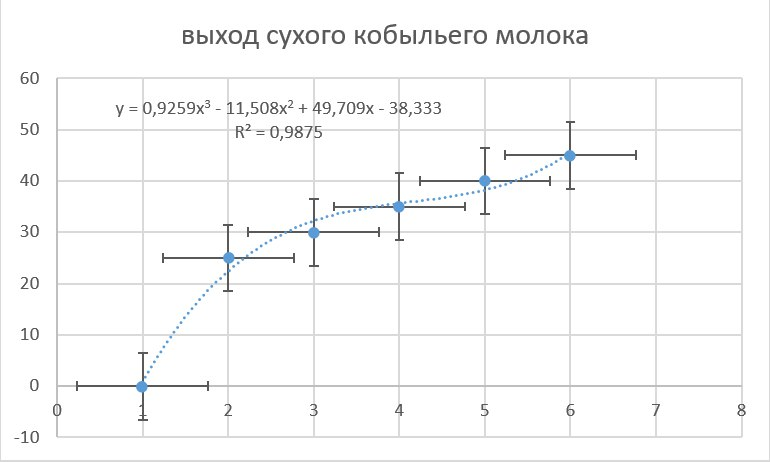
\includegraphics[width=0.8\textwidth]{assets/309-6}
	\caption*{Рис. 1 -- Выход сухого молока в зависимости от температуры}
\end{figure}


\begin{multicols}{2}

На представленной диаграмме (рис.1) изображена зависимость выхода сухого
кобыльего молока от времени или других экспериментальных условий (ось
X), где по оси Y обозначен выход продукта в граммах. График имеет форму
полинома третьей степени (кубическая кривая), уравнение которой
представлено как:

\(y = {0.926x}^{3} - 11.508x^{2} + 49.7x - 38.33\) (1)

где y -- выход сухого молока, x -- время или другие условия
эксперимента.

Значение коэффициента детерминации R\textsuperscript{2}=0.9875 указывает
на высокую степень соответствия модели экспериментальным данным.
Наблюдается увеличение выхода сухого молока по мере увеличения значения
оси X до определенной точки, после чего рост стабилизируется или
замедляется. График показывает, что на начальных стадиях эксперимента
прирост выхода продукта наиболее интенсивный, затем он становится более
плавным.

График содержит ошибки (погрешности) измерений, представленные в виде
горизонтальных и вертикальных отрезков. Вертикальные отрезки показывают
вариации в выходе сухого молока, что может быть связано с
экспериментальными неточностями или естественной вариативностью
образцов. Горизонтальные отрезки указывают на вариации значений оси X,
что также может отражать экспериментальные условия.

Из анализа графика следует, что существует оптимальная область значений
оси X, при которых выход сухого молока максимален и стабилен. Это
подтверждается стабилизацией кривой после определенного значения.
Дальнейшее увеличение значения X приводит к снижению прироста выхода,
что может свидетельствовать о достижении предела эффективности данного
метода сублимационной сушки. Присутствие погрешностей указывает на
необходимость учёта возможных отклонений в экспериментальных условиях и
повторяемости результатов. Это важно для будущих исследований и
масштабирования процесса. На основе полученных данных, рекомендуется
проводить дальнейшие эксперименты в пределах оптимальной области
значений оси X, чтобы максимизировать выход сухого молока и
минимизировать затраты.

Необходимо также учитывать и минимизировать экспериментальные
погрешности для повышения точности и повторяемости результатов.

Таким образом, проведенный анализ демонстрирует успешность выбранного
метода и указывает на возможности дальнейшей оптимизации процесса
сублимационной сушки для повышения выхода сухого кобыльего молока.

\emph{Параметры при сушке кобыльего молока на сублимационной установке
(Майкудук)}

Процесс сушки был проведен при различных параметрах температуры полок и
давления в камере. В таблице 2 приведены основные параметры:

\end{multicols}


\begin{longtable}[H]{|p{(\columnwidth - 14\tabcolsep) * \real{0.1457}}|
  p{(\columnwidth - 14\tabcolsep) * \real{0.2341}}|
  p{(\columnwidth - 14\tabcolsep) * \real{0.1698}}|
  p{(\columnwidth - 14\tabcolsep) * \real{0.0902}}|
  p{(\columnwidth - 14\tabcolsep) * \real{0.0901}}|
  p{(\columnwidth - 14\tabcolsep) * \real{0.0901}}|
  p{(\columnwidth - 14\tabcolsep) * \real{0.0901}}|
  p{(\columnwidth - 14\tabcolsep) * \real{0.0901}}|}
\caption*{Таблица 2- Параметры при сушке кобыльего молока на сублимационной сушке (Майкудук)}\\
\hline
\begin{minipage}[b]{\linewidth}\raggedright
Время
\end{minipage} & \begin{minipage}[b]{\linewidth}\raggedright
Показатели
\end{minipage} & \begin{minipage}[b]{\linewidth}\raggedright
Ед. измерения
\end{minipage} &
\multicolumn{5}{>{\raggedright\arraybackslash}p{(\columnwidth - 14\tabcolsep) * \real{0.4504} + 8\tabcolsep}|}{%
\begin{minipage}[b]{\linewidth}\raggedright
Значения
\end{minipage}} \\
\hline
\endhead
\hline
\endfoot
\hline
\multirow{3}{*}{09.30} & Температура полок & С° & 24.7 & 29.6 & 34.7 & 39.9 & 44.6 \\
\hline
& Давление в камере & Па & 57.8 & 57.8 & 57.8 & 57.8 & 57.8 \\
\hline
& Температура десублиматора & С° & -23.9 & -23.9 & -23.9 & -23.9 & -23.9 \\
\hline
\multirow{3}{*}{09.34} & Температура полок & С° & 24.7 & 29.7 & 34.8 & 39.7 & 44.9 \\
\hline
& Давление в камере & Па & 65.1 & 65.1 & 65.1 & 65.1 & 65.1 \\
\hline
& Температура десублиматора & С° & -24.1 & -24.1 & -24.1 & -24.1 & -24.1 \\
\hline
\multirow{3}{*}{09.38} & Температура полок & С° & 24.8 & 29.9 & 34.9 & 39.6 & 44.4 \\
\hline
& Давление в камере & Па & 70.0 & 70.0 & 70.0 & 70.0 & 70.0 \\
\hline
& Температура десублиматора & С° & -24.1 & -24.1 & -24.1 & -24.1 & -24.1 \\
\hline
\multirow{3}{*}{09.44} & Температура полок & С° & 24.8 & 29.8 & 34.7 & 39.9 & 44.6 \\
\hline
& Давление в камере & Па & 80.2 & 80.2 & 80.2 & 80.2 & 80.2 \\
\hline
& Температура десублиматора & С° & -24.3 & -24.3 & -24.3 & -24.3 & -24.3 \\
\hline
\multirow{3}{*}{09.51} & Температура полок & С° & 24.5 & 29.7 & 34.6 & 39.7 & 44.8 \\
\hline
& Давление в камере & Па & 90.2 & 90.2 & 90.2 & 90.2 & 90.2 \\
\hline
& Температура десублиматора & С° & -24.4 & -24.4 & -24.4 & -24.4 & -24.4 \\
\hline
\multirow{3}{*}{09.57} & Температура полок & С° & 24.7 & 29.8 & 34.8 & 39.5 & 44.8 \\
\hline
& Давление в камере & Па & 99.2 & 99.2 & 99.2 & 99.2 & 99.2 \\
\hline
& Температура десублиматора & С° & -24.6 & -24.6 & -24.6 & -24.6 & -24.6 \\
\hline
\multirow{3}{*}{09.58} & Температура полок & С° & 24.5 & 29.6 & 34.9 & 39.5 & 44.9 \\
\hline
& Давление в камере & Па & 100 & 100 & 100 & 100 & 100 \\
\hline
& Температура десублиматора & С° & -24.6 & -24.6 & -24.6 & -24.6 & -24.6 \\
\hline
\multirow{3}{*}{10.00} & Температура полок & С° & 24.7 & 29.9 & 34.5 & 39.6 & 44.7 \\
\hline
& Давление в камере & Па & 49.3 & 49.3 & 49.3 & 49.3 & 49.3 \\
\hline
& Температура десублиматора & С° & -24.6 & -24.6 & -24.6 & -24.6 & -24.6 \\
\hline
\multirow{3}{*}{10.02} & Температура полок & С° & 24.6 & 29.8 & 34.9 & 39.9 & 44.5 \\
\hline
& Давление в камере & Па & 50.1 & 50.1 & 50.1 & 50.1 & 50.1 \\
\hline
& Температура десублиматора & С° & -24.6 & -24.6 & -24.6 & -24.6 & -24.6 \\
\hline
\multirow{3}{*}{10.8} & Температура полок & С° & 24.7 & 29.8 & 34.8 & 39.6 & 44.8 \\
\hline
& Давление в камере & Па & 60.0 & 60.0 & 60.0 & 60.0 & 60.0 \\
\hline
& Температура десублиматора & С° & -25.0 & -25.0 & -25.0 & -25.0 & -25.0 \\
\hline
\multirow{3}{*}{09.29} & Температура полок & С° & 24.6 & 29.6 & 34.9 & 39.7 & 44.7 \\
\hline
& Давление в камере & Па & 79.4 & 79.4 & 79.4 & 79.4 & 79.4 \\
\hline
& Температура десублиматора & С° & -26.8 & -26.8 & -26.8 & -26.8 & -26.8 \\
\hline
\end{longtable}

\begin{multicols}{2}

Для оценки значимости различий в температурах полок был проведен
дисперсионный анализ (ANOVA). Результаты анализа показали следующие
значения: F-значение= 38069.58, p-значение= 2.09e\textsuperscript{-86}.
Значение p-значения (2.09e-86) значительно меньше уровня значимости
0.05, что указывает на высокую статистическую значимость различий между
температурами полок. Высокое F-значение (38069.58) подтверждает наличие
существенных различий в температурах полок в разные временные интервалы.
Соответственно, значительные различия в температурах полок указывают на
то, что различные температурные режимы оказывают значительное влияние на
процесс сублимационной сушки.

{\bfseries Выводы.} Результаты подтверждают важность тщательного контроля
температурного режима полок и давления в камере для обеспечения
максимального выхода и качества сухого кобыльего молока. Это согласуется
с выводами из статей 2024 года, таких как работы в {[}10{]} и {[}11{]},
которые подчеркивают значимость оптимальных условий для сохранения
биологически активных компонентов молока.

Оптимальные параметры сублимационной сушки:

Оптимальные температуры полок (34.7°C - 39.9°C) и стабильное давление
(57.8 Па - 100 Па) обеспечивают максимальный выход сухого молока и
сохранение его качественных характеристик. Эти данные подтверждаются
исследованиями, представленными в специальных выпусках и статьях{[}10,
12{]}.

Практическое применение результатов:

Результаты исследования могут быть использованы для оптимизации
промышленного процесса производства сухого кобыльего молока. Это
подтверждается работами, опубликованными в 2024 году, которые
подчеркивают значимость правильного выбора технологических параметров
для улучшения качества конечного продукта.

Дальнейшие исследования:

Для уточнения оптимальных параметров процесса сублимационной сушки и
изучения их влияния на сохранение питательных и биологически активных
компонентов кобыльего молока необходимы дальнейшие исследования.

Таким образом выводы и рекомендации согласуются с существующей научной
литературой, подтверждая эффективность и важность выбранных методов для
производства качественного сухого кобыльего молока

{\bfseries Рекомендации}

\begin{itemize}
\item
  для обеспечения максимального выхода сухого молока рекомендуется
  поддерживать температуру полок в пределах 34.7°C - 39.9°C.
\item
  необходимо поддерживать давление в камере в пределах 57.8 Па - 100 Па
  для обеспечения стабильного процесса сушки.
\item
  температура десублиматора должна оставаться в диапазоне от -23.9°C до
  -26.8°C для сохранения качественных характеристик молока.
\item
  рекомендуется проведение дальнейших исследований для уточнения
  оптимальных параметров процесса сублимационной сушки и изучения их
  влияния на сохранение питательных и биологически активных компонентов
  кобыльего молока.
\end{itemize}

Таким образом, представленные данные и их анализ дают четкое понимание о
ключевых параметрах процесса сублимационной сушки кобыльего молока, что
способствует улучшению его эффективности и качества.

\emph{{\bfseries Финансирование.} Данное исследование
финансировалось/финансируется Комитетом по науке Министерства науки и
высшего образования Республики Казахстан (грант № BR21881957 Разработка
технологии глубокой переработки и оборудования вакуум-сублимационной
сушки кобыльего и верблюжьего молока.}

\end{multicols}

\begin{center}
  {\bfseries Литература}
  \end{center}


  \begin{noparindent}

1. Salimei E., Fantuz F. Equid milk for human consumption //
International Dairy Journal. -2012. -Vol. 24(2), -P. 130-142. DOI
10.1016/J.IDAIRYJ.2011.11.008

2. Teichert J., Cais-Sokolińska D., Danków R., Pikul J. Color stability
of fermented mare\textquotesingle s milk and a fermented beverage from
cow\textquotesingle s milk adapted to mare\textquotesingle s milk
composition. Foods. mdpi.com. -2020. --Vol. 9(2). DOI
10.3390/foods9020217

3. Miraglia, N., Salimei, E., \& Fantuz, F. Equine milk production and
valorization of marginal areas-A review. Animals. mdpi.com. -2020.
--Vol. 10(2). DOI 10.3390/ani10020353

4. Ratti, C. Hot air and freeze-drying of high-value foods: A review //
Journal of Food Engineering, -2001. --Vol. 49(4). --P. 311-319. DOI
10.1016/S0260-8774(00)00228-4

5. Cais-Sokolińska, D., Teichert, J., \& Gawałek, J. Foaming and other
functional properties of freeze-dried mare\textquotesingle s milk.
Foods. mdpi.com. -2023. --Vol. 12(11). DOI 10.3390/foods12112274

6. Kondybayev, A., Loiseau, G., Achir, N., Mestres, C., \& Shaikh, A.
Fermented mare milk product (Qymyz, Koumiss) // International Dairy
Journal. Elsevier. -2021. --Vol. 119.\\ DOI 10.1016/J.IDAIRYJ.2021.105065

7. Simonenko E.S., Begunova A.V. Development of fermented milk product
based on mare milk and lactic microorganisms association. Vopr Pitan.
voprosy-pitaniya.ru. -2021. --Vol. 90(5). --P. 115-125 DOI
10.33029/0042-8833-2021-90-5-115-125

8. Baibokonov, D., Yang, Y., \& Tang, Y. Understanding the traditional
mares\textquotesingle{} milk industry\textquotesingle s transformation
into a creative industry: Empirical evidence from Kazakhstan // Growth
and Change. -2021. --Vol. 52(1). DOI10.1111/grow.12478

9. Hinz, K., O'Connor, P. M., Huppertz, T., Ross, R. P., \& Kelly, A. L.
Comparison of the principal proteins in bovine, caprine, buffalo, equine
and camel milk // Journal of Dairy Research. -2012. --Vol. 79(2). --P.
185-191. DOI10.1017/s0022029912000015

10. Cais-Sokolińska D., Teichert J., Gawałek J. Foaming and Other
Functional Properties of Freeze-Dried Mare's Milk // Foods. -2024.
--Vol. 12(11). https://doi.org/10.3390/foods12112274

11. Milkify\textquotesingle s Freeze-Drying Benefits // Milkify. -2024.
URL: https://www.milkify.me

12. Bhatta S., Stevanovic Janezic T., Ratti, C. Freeze-Drying of
Plant-Based Foods // Foods. -2024. --Vol. 9. DOI10.3390/foods9010087.

\end{noparindent}

\emph{{\bfseries Сведения об авторах}}

\begin{noparindent}

Рахматулина А.Б.- PhD, доцент, Отдел машиноведения и робототехники
Институт механики и \\машиноведения имени академика У. А. Джолдасбекова,
Алматы, Казахстан, e-mail: kazrah@mail.ru;

Диханбаева Ф.Т. -- доктор технических наук, профессор кафедры
«Технология продуктов питания», Алматинский технологический университет,
Институт механики и машиноведения имени академика У. А. Джолдасбекова,
Алматы, Казахстан, е-mail: fatima6363@mail.ru;

Тлевлесова Д.А.-- PhD, ассоциированный профессор, ТОО «КазНИИППП»,
Институт механики и машиноведения имени академика У. А. Джолдасбекова,
Алматы, Казахстан, \\e-mail: tlevlessova@gmail.com;

Изтилеуов М.К.-магистр., Алматинский технологический университет,
Алматы, Казахстан, еmail: m.iztileuov@mail.ru;

Калемшарив Б. -- докторант, Казахский агротехнический исследовательский
университет им. \\С. Сейфуллина, Астана, Казахстан, е-mail:
begjan.ae@gmail.com.

\end{noparindent}

\emph{{\bfseries Information about authors}}

\begin{noparindent}

Rakhmatulina A.B. -- PhD, Associate Professor, Institute of Mechanics
and Engineering named after Academician U.A. Zholdasbekov, Almaty,
Kazakhstan, e-mail: kazrah@mail.ru;

Dikhanbaeva F.T. -- Doctor of Technical Sciences, Professor, Department
of "Food Technology," Almaty Technological University, Institute of
Mechanics and Engineering named after Academician \\U.A. Zholdasbekov,
Almaty, Kazakhstan, e-mail: fatima6363@mail.ru;

Tlevlessova D.A. -- PhD, Associate Professor, LLP "KazNII PPP,"
Institute of Mechanics and Engineering named after Academician U.A.
Zholdasbekov, Almaty, Kazakhstan, e-mail: tlevlessova@gmail.com;

Iztileuov M.K. -- Master's Degree, Almaty Technological University,
Almaty, Kazakhstan, \\e-mail: m.iztileuov@mail.ru;

Kalemshariv B. -- Doctoral Candidate, Kazakh Agrotechnical Research
University named after S. Seifullin, Astana, Kazakhstan, e-mail:
begjan.ae@gmail.com.

\end{noparindent}



























